\documentclass[aspectratio=169,12pt]{beamer}
\mode<presentation> {
  \usetheme{metropolis}
}

\usepackage{lipsum}
\usepackage[colorgrid,gridunit=pt,texcoord]{eso-pic}
\usepackage[absolute,overlay]{textpos}
\usepackage{pythonhighlight}
\usepackage[absolute,overlay]{textpos}
\usepackage{url}
\usepackage{caption}
\usepackage{hyperref}
\usepackage[
    type={CC},
    modifier={by},
    version={3.0},
]{doclicense}
\usepackage{emoji}
\setemojifont{TwemojiMozilla}

\setbeamertemplate{note page}{\pagecolor{yellow!5}\vfill\insertnote\vfill}
\setbeameroption{show notes on second screen=right}

\lstset{
language = Python,
breaklines = true,
basicstyle=\fontsize{7}{7}\selectfont\ttfamily,
commentstyle = {\itshape \color[cmyk]{1,0.4,1,0}},
keywordstyle = {\bfseries \color[cmyk]{0,1,0,0}},
stringstyle = {\ttfamily \color[rgb]{1,0,0}},
frame = single,
}
\hypersetup{
colorlinks=true,
}

\title{Visualize 3D scientific data in a Pythonic way like matplotlib}

\begin{document}
\author{Tetsuo Koyama}
\institute{PyVista developer team}
\date{Scipy 2021}

\frame{\titlepage}

\begin{frame}[fragile]
\begin{textblock*}{350pt}(50pt, 20pt)
\begin{block}{Who am I?}
\note{Let me introduce myself first.}
\note{My Twitter and Github accounts are \href{https://twitter.com/tkoyama010}{@tkoyama010}.}
\note{Please follow me if you like this presentation.}
\end{block}
\end{textblock*}
\begin{textblock*}{350pt}(50pt, 70pt)

\includegraphics[width=0.25\linewidth]{tkoyama010.png}
\end{textblock*}
\begin{textblock*}{350pt}(50pt, 170pt)

\includegraphics[width=0.05\linewidth]{twitter-5662063_1280.png}
\end{textblock*}
\begin{textblock*}{350pt}(70pt, 175pt)
\href{https://twitter.com/tkoyama010}{@tkoyama010}
\end{textblock*}
\begin{textblock*}{350pt}(50pt, 200pt)

\includegraphics[width=0.05\linewidth]{github.png}
\end{textblock*}
\begin{textblock*}{350pt}(70pt, 205pt)
\href{https://github.com/tkoyama010}{@tkoyama010}
\end{textblock*}
\begin{textblock*}{350pt}(150pt, 25pt)
\begin{itemize}
\item \emoji{gear} Mechanical simulation software engineer.
\item \emoji{japan} Stuff of Scipy Japan 2020.
\item \emoji{computer} PyVista developer team member.
\item \emoji{heart} Science Python Anime and Manga.
\end{itemize}
\end{textblock*}
\begin{textblock*}{350pt}(200pt, 120pt)
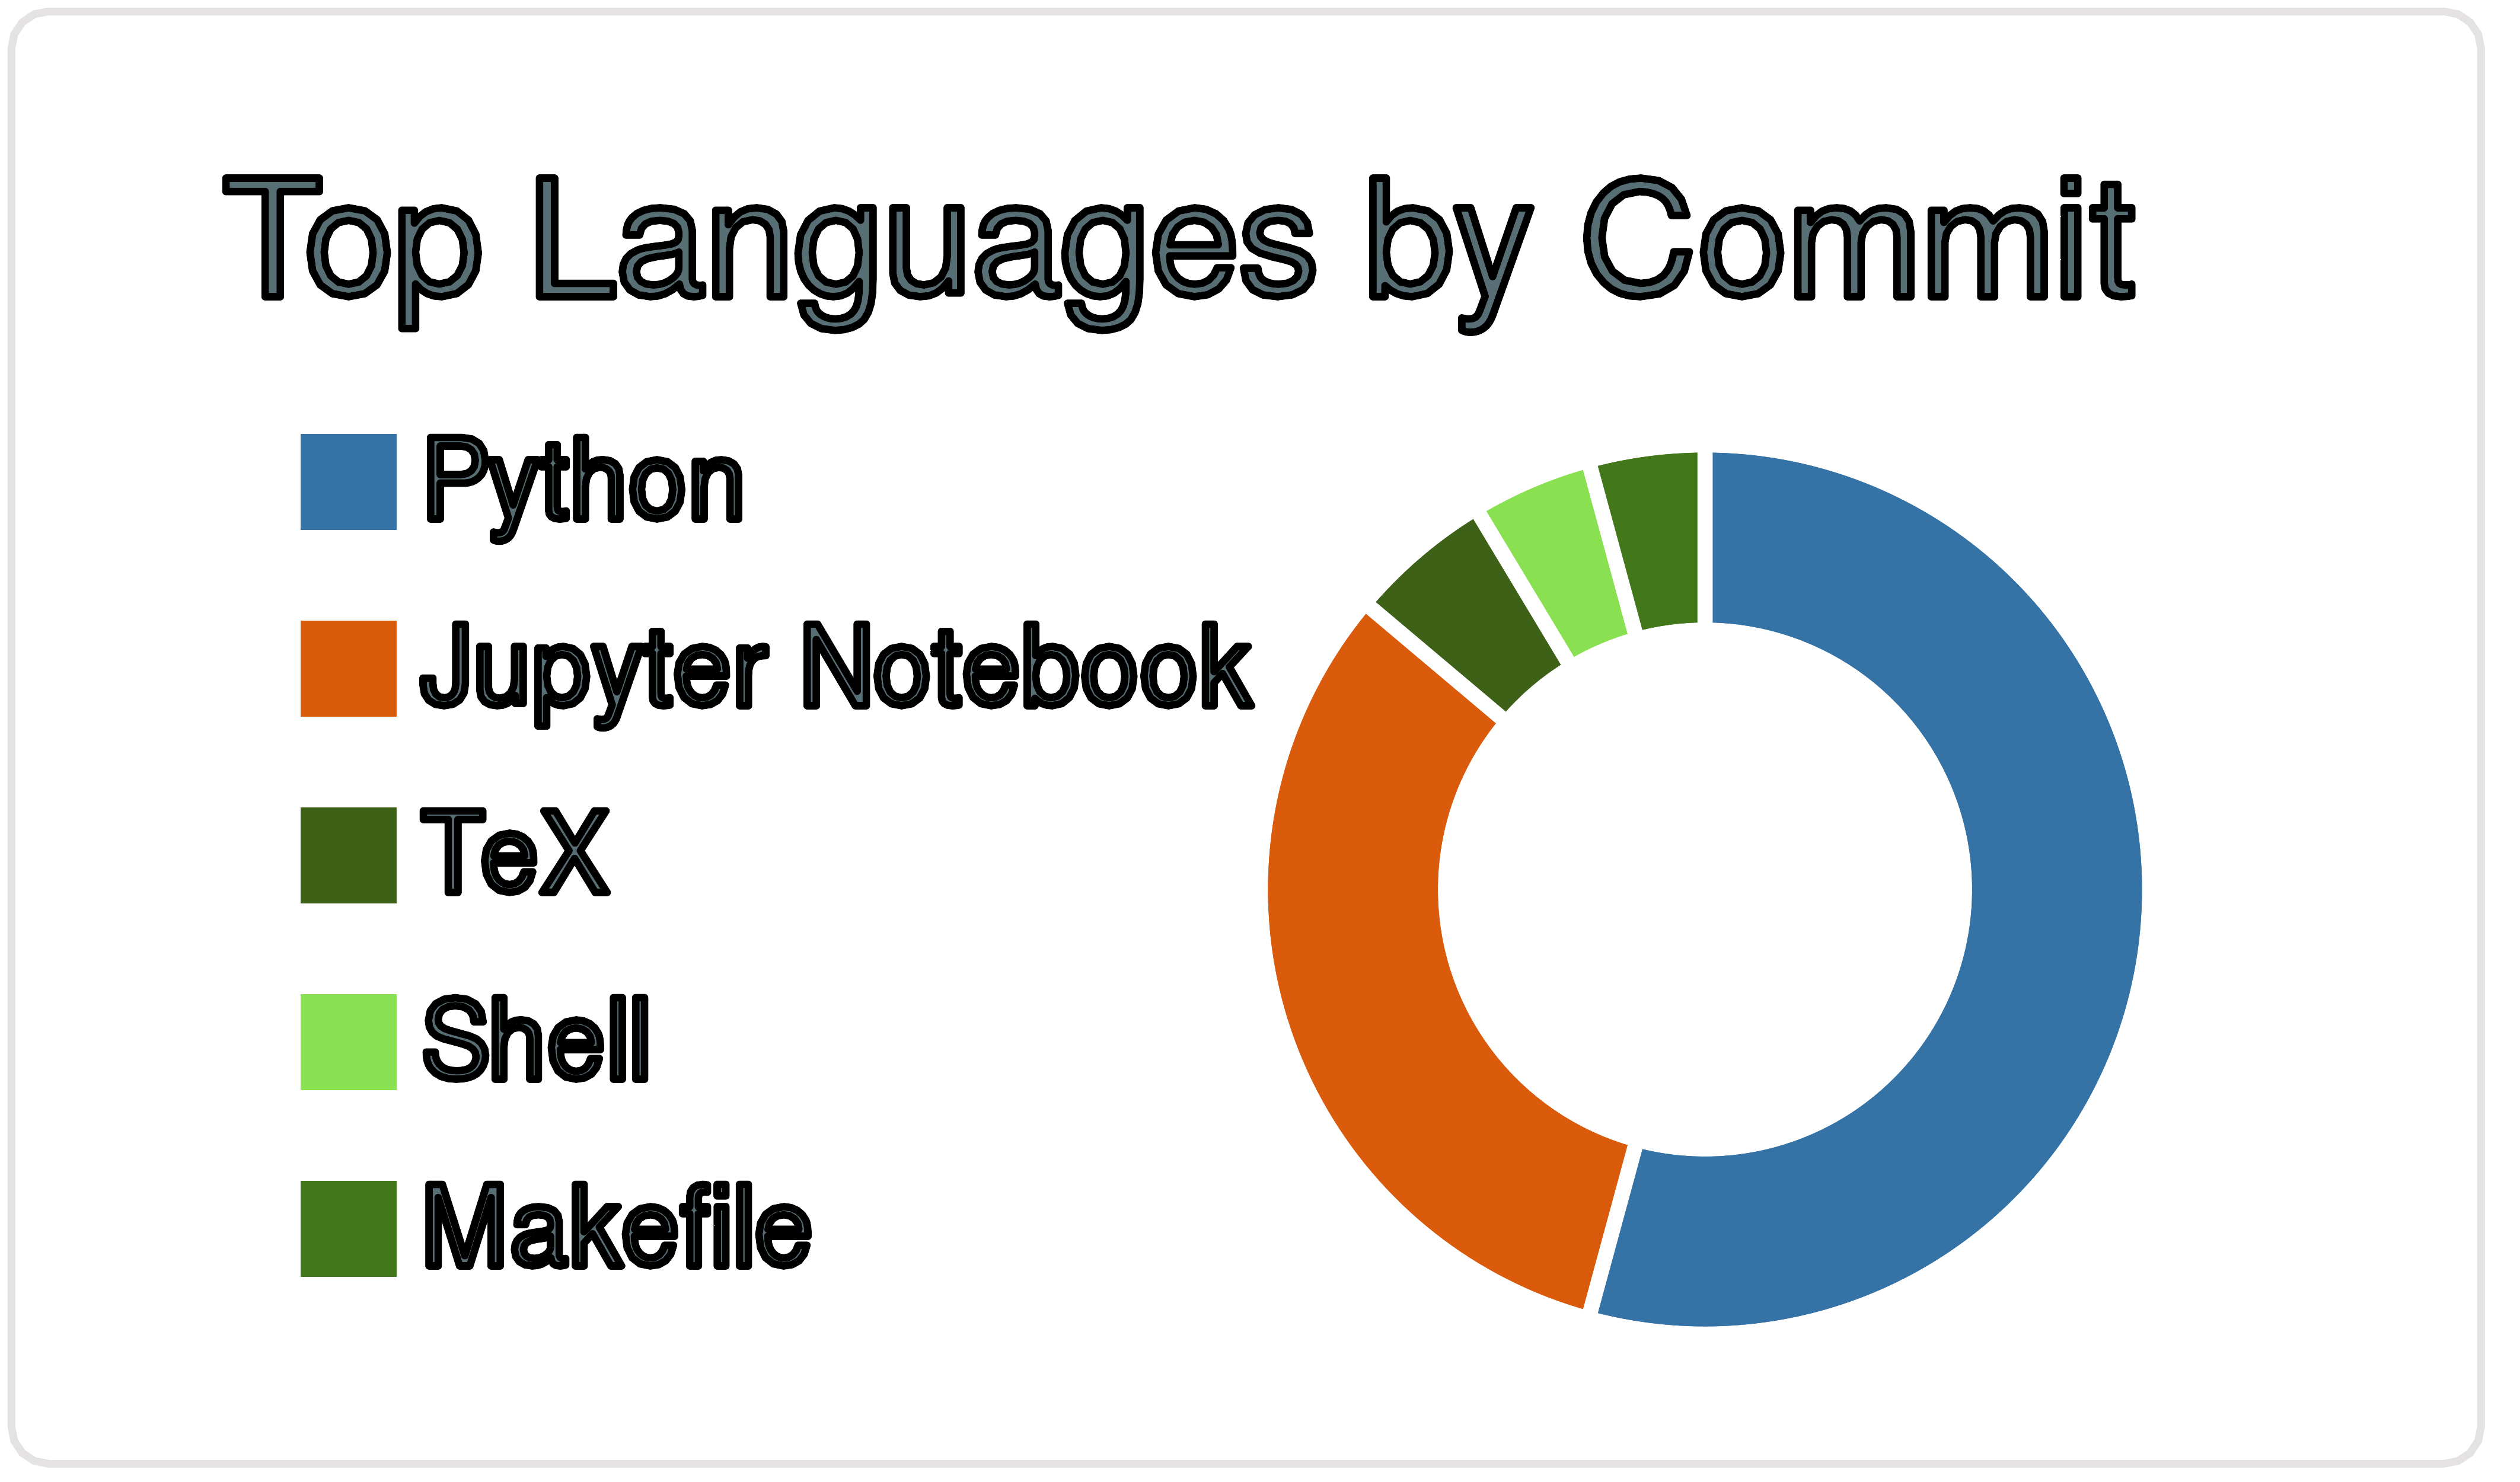
\includegraphics[width=0.50\linewidth]{2-most-commit-language.png}
\end{textblock*}
\end{frame}

\begin{frame}[fragile]
\begin{textblock*}{800pt}(50pt, 20pt)
\begin{block}{Overview}
\note{Do you want to visualize 3D scientific data in a Pythonic way like matplotlib?}
\note{If you want, this slides is for you.}
\note{This slides is the introduction of \href{https://pypi.org/project/pyvista/}{PyVista}.}
\note{It is}
\begin{itemize}
\item "VTK for humans"\: a high-level API to the Visualization Toolkit (VTK)
\note[item]{"VTK for humans"\: a high-level API to the Visualization Toolkit (VTK)}
\item 3D plotting made simple and built for large/complex data geometries
\note[item]{3D plotting made simple and built for large/complex data geometries}
\item mesh data structures and filtering methods for spatial datasets
\note[item]{mesh data structures and filtering methods for spatial datasets}
\end{itemize}
\end{block}
\end{textblock*}
\begin{textblock*}{800pt}(50pt, 100pt)
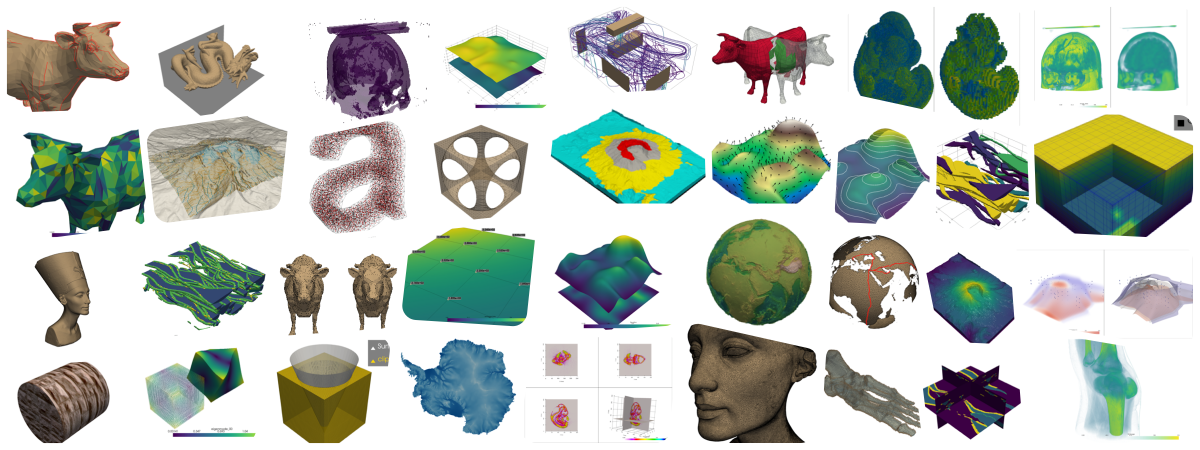
\includegraphics[width=0.50\linewidth]{pyvista_banner_small.png}
\end{textblock*}
\end{frame}

\begin{frame}[fragile]
\begin{textblock*}{350pt}(50pt, 10pt)
\begin{block}{Hello World!}
\note{In Code Listing \ref{hello_world_code}, we demonstrate the "Hello World!" of \href{https://pypi.org/project/pyvista/}{PyVista}.}
\note{Basic step of \href{https://pypi.org/project/pyvista/}{PyVista} script is the following.}
\note{First, import \href{https://pypi.org/project/pyvista/}{PyVista}.}
\note{Then generate \href{https://dev.pyvista.org/getting-started/what-is-a-mesh.html}{mesh} and add it to}
\note{Plotter object using add mesh method.}
\lstinputlisting[caption=Hello World!, label=hello_world_code, firstline=1, lastline=100]{hello_world.py}
\end{block}
\end{textblock*}
\end{frame}

\begin{frame}[fragile]
\begin{textblock*}{350pt}(50pt, 10pt)
\begin{block}{Hello World!}
\end{block}
\end{textblock*}
\begin{textblock*}{350pt}(50pt, 50pt)
\begin{block}{}
\begin{figure}
\includegraphics[width=1.0\linewidth]{hello_world.png}
\caption{Hello World!\label{HelloWorldFigure}}
\end{figure}
\note{And finally, we can check the render view (Figure \ref{HelloWorldFigure}) of PyVista using show method.}
\end{block}
\end{textblock*}
\end{frame}

\begin{frame}[fragile]
\begin{textblock*}{350pt}(50pt, 10pt)
\begin{block}{General filters to any data type}

\lstinputlisting[caption=Shrink Mesh, label=ShrinkFilterCode, firstline=4, lastline=5]{shrunk_mesh.py}
\begin{figure}
\includegraphics[width=1.0\linewidth]{shrink.png}
\caption{Shrink filter\label{ShrinkFilterFigure}}
\end{figure}
\note{\href{https://dev.pyvista.org/core/filters.html}{PyVista classes} hold methods to apply general filters to any data type.}
\note{A user can easily apply common filters in an intuitive manner.}
\note{For example,}
\note{Code Listing \ref{ShrinkFilterCode} shrink the individual faces of a mesh}
\note{using shrink method (Figure \ref{ShrinkFilterFigure}), and}
\end{block}
\end{textblock*}
\end{frame}

\begin{frame}[fragile]
\begin{textblock*}{350pt}(50pt, 10pt)
\begin{block}{Rotation about the x axis}
\note{Rotations of a mesh about its axes. In this model, the x axis is from the left}
\note{to right; the y axis is from bottom to top; and the z axis emerges from the}
\note{image. The camera location is the same in all four images.}
\note{Plot the mesh rotated about the x axis every 60 degrees.}
\note{Add the axes actor to the Plotter and set the axes origin to the point of rotation.}
\end{block}
\lstinputlisting[caption=X-Axis Rotation, firstline=66, lastline=69]{rotate.py}
\begin{figure}
\includegraphics[width=1.0\linewidth]{rotate_y.png}
\caption{X-Axis Rotation}
\end{figure}
\end{textblock*}
\end{frame}

\begin{frame}[fragile]
\begin{textblock*}{350pt}(50pt, 10pt)
\begin{block}{Rotation about the y axis}
\note{Plot the mesh rotated about the y axis every 60 degrees.}
\note{Add the axes actor to the Plotter and set the axes origin to the point of rotation.}
\end{block}
\lstinputlisting[caption=X-Axis Rotation, firstline=66, lastline=69]{rotate.py}
\begin{figure}
\includegraphics[width=1.0\linewidth]{rotate_x.png}
\caption{X-Axis Rotation}
\end{figure}
\end{textblock*}
\end{frame}

\begin{frame}[fragile]
\begin{textblock*}{350pt}(50pt, 10pt)
\begin{block}{Rotation about the z axis}
\note{Plot the mesh rotated about the z axis every 60 degrees.}
\note{Add the axes actor to the Plotter and set the axes origin to the point of rotation.}
\end{block}
\lstinputlisting[caption=X-Axis Rotation, firstline=66, lastline=69]{rotate.py}
\begin{figure}
\includegraphics[width=1.0\linewidth]{rotate_x.png}
\caption{X-Axis Rotation}
\end{figure}
\end{textblock*}
\end{frame}

\begin{frame}[fragile]
\begin{textblock*}{350pt}(50pt, 10pt)
\begin{block}{Rotation about a custom vector}
\note{Plot the mesh rotated about a custom vector every 60 degrees.}
\note{Add the axes actor to the Plotter and set axes origin to the point of rotation.}
\end{block}
\lstinputlisting[caption=X-Axis Rotation, firstline=66, lastline=69]{rotate.py}
\begin{figure}
\includegraphics[width=1.0\linewidth]{rotate_x.png}
\caption{X-Axis Rotation}
\end{figure}
\end{textblock*}
\end{frame}

\begin{frame}[fragile]
\begin{textblock*}{350pt}(50pt, 10pt)
\begin{block}{General filters to any data type}
\lstinputlisting[caption=Extrude Rotate, label=ExtrudeRotateCode, firstline=7, lastline=9]{extrude_rotate.py}
\begin{figure}
\includegraphics[width=1.0\linewidth]{extrude_rotate.png}
\caption{Extrude Rotation\label{ExtrudeRotateFigure}}
\end{figure}
\note{Code Listing \ref{ExtrudeRotateCode} sweep polygonal data creating "skirt" from line}
\note{using extrude rotate method (Figure \ref{ExtrudeRotateFigure}).}
\end{block}
\end{textblock*}
\end{frame}

\begin{frame}[fragile]
\begin{textblock*}{350pt}(50pt, 10pt)
\begin{block}{Load and plot from a files}
\lstinputlisting[caption=Load meshs from the many supported file formats, label=ReadFileCode, firstline=5, lastline=8]{read_file.py}
\begin{figure}
\includegraphics[width=0.6\linewidth]{read_file.png}
\caption{Meshs from the many supported file formats\label{ReadFileFigure}}
\end{figure}
\note{Loading a \href{https://dev.pyvista.org/getting-started/what-is-a-mesh.html}{mesh} is trivial - if your data is in one of the many supported file formats,}
\note{simply use \href{https://dev.pyvista.org/utilities/utilities.html}{pyvista.read()}}
\note{to load your spatially referenced dataset into a \href{https://pypi.org/project/pyvista/}{PyVista} \href{https://dev.pyvista.org/getting-started/what-is-a-mesh.html}{mesh} object}
\note{(Code Listing \ref{ReadFileCode}, Figure \ref{ReadFileFigure}).}
\end{block}
\end{textblock*}
\end{frame}

\begin{frame}[fragile]
\begin{textblock*}{350pt}(50pt, 10pt)
\begin{block}{Load and plot from a files}
\lstinputlisting[caption=Save meshs to the many supported file formats, label=SaveFileCode, firstline=26, lastline=29]{read_file.py}
\begin{figure}
\includegraphics[width=0.6\linewidth]{read_file.png}
\caption{Meshs from the many supported file formats\label{ReadFileFigure}}
\end{figure}
\note{Also note that we can export any \href{https://pypi.org/project/pyvista/}{PyVista} mesh to any file format supported by \href{https://pypi.org/project/meshio/}{meshio}.}
\note{To save a \href{https://pypi.org/project/pyvista/}{PyVista} mesh using meshio, use \href{https://dev.pyvista.org/utilities/utilities.html}{pyvista.save\_meshio()}(Code Listing \ref{SaveFileCode}):}
\end{block}
\end{textblock*}
\end{frame}

\begin{frame}[fragile]
\begin{textblock*}{350pt}(50pt, 10pt)
\begin{block}{Extracting and Contouring}
\lstinputlisting[caption=Extracted by scalar, label=WarpScalarCode, firstline=9, lastline=9]{contour.py}
\begin{figure}
\includegraphics[width=0.5\linewidth]{contour.png}
\caption{Contouring\label{WarpScalarFigure}}
\end{figure}
\note{Attributes are data values that live on either the nodes or cells of a mesh.}
\note{In \href{https://pypi.org/project/pyvista/}{PyVista}, we work with both point data and cell data and allow easy access to data dictionaries to hold arrays for attributes that live either on all nodes or on all cells of a mesh.}
\note{Meshes can have a scalar field extracted}
\note{using \href{https://dev.pyvista.org/core/filters.html}{warp\_by\_scalar()} method}
\note{(Code List \ref{WarpScalarCode}, Figure \ref{WarpScalarFigure}).}
\note{Also can have a vector filed extracted}
\note{using \href{https://dev.pyvista.org/core/filters.html}{warp\_by\_vector()} method}
\note{(Code List \ref{WarpVectorCode}, Figure \ref{WarpVectorFigure}).}
\note{\href{https://dev.pyvista.org/plotting/plotting.html}{add\_mesh()} method can use a Matplotlib, Colorcet, cmocean, or custom colormap when plotting scalar values}
\note{(Figure \ref{WarpVectorFigure}).}
\end{block}
\end{textblock*}
\end{frame}

\begin{frame}[fragile]
\begin{textblock*}{350pt}(50pt, 10pt)
\begin{block}{Extracting and Contouring}
\lstinputlisting[caption=Extracted by vector, label=WarpVectorCode, firstline=44, lastline=44]{contour.py}
\begin{figure}
\includegraphics[width=1.0\linewidth]{warped_vector.png}
\caption{Warped sphere by vector\label{WarpVectorFigure}}
\end{figure}
\end{block}
\end{textblock*}
\end{frame}

\begin{frame}[fragile]
\begin{textblock*}{350pt}(50pt, 10pt)
\begin{block}{Camera class}
\begin{figure}
\includegraphics[width=0.75\linewidth]{frustum_of_camera.png}
\caption{Frustum of camera \label{CameraFrustumFigure}}
\end{figure}
\note{\href{https://dev.pyvista.org/core/camera.html}{Camera} class is a virtual camera for 3D rendering.}
\note{It provides methods to position and orient the view point and focal point.}
\note{Convenience methods for moving about the focal point also are provided.}
\note{More complex methods allow the manipulation of the computer graphics model including view up vector, clipping planes, and camera perspective (Figure \ref{CameraFrustumFigure}).}
\note{Code Listing \ref{CameraFrustumCode} create a camera and frustum.}
\note{Then create a scene of inside frustum adding \href{https://dev.pyvista.org/core/camera.html}{Camera} object to \href{https://dev.pyvista.org/plotting/plotting.html}{Plotter} object}
\note{(Code list \ref{CameraFrustumCode} ,Figure \ref{CameraFrustumFigure}).}
\lstinputlisting[caption=Add Camera to Plotter, label=camera_view, firstline=7, lastline=13]{camera_view.py}
\end{block}
\end{textblock*}
\end{frame}

\begin{frame}[fragile]
\begin{textblock*}{350pt}(50pt, 10pt)
\begin{block}{Camera class}
\lstinputlisting[caption=Create camera frustum, label=CameraFrustumCode, firstline=8, lastline=13]{frustum_of_camera.py}
\begin{figure}
\includegraphics[width=0.75\linewidth]{camera_view.png}
\caption{Camera view}
\end{figure}
\end{block}
\end{textblock*}
\end{frame}

\begin{frame}[fragile]
\begin{textblock*}{150pt}(50pt, 10pt)
\begin{block}{Controlling Camera Rotation}
\lstinputlisting[caption=Controlling Camera Rotation, label=CameraRotationCode, firstline=29, lastline=29]{camera_view.py}
\lstinputlisting[firstline=34, lastline=34]{camera_view.py}
\lstinputlisting[firstline=39, lastline=39]{camera_view.py}
\end{block}
\end{textblock*}
\begin{textblock*}{350pt}(150pt, 50pt)
\begin{figure}
\includegraphics[width=0.5\linewidth]{camera_rotation.png}
\caption{Controlling Camera Rotation \label{CameraRotationFigure}}
\end{figure}
\note{In addition to directly controlling the camera position by setting it via the pyvista.}
\note{\href{https://dev.pyvista.org/core/camera.html}{Camera.position}}
\note{property, you can also directly control the}
\note{\href{https://dev.pyvista.org/core/camera.html}{pyvista.Camera.roll},}
\note{\href{https://dev.pyvista.org/core/camera.html}{pyvista.Camera.elevation}, and}
\note{\href{https://dev.pyvista.org/core/camera.html}{pyvista.Camera.azimuth}}
\note{of the camera.}
\note{(Code list \ref{CameraRotationCode} ,Figure \ref{CameraRotationFigure}).}
\end{textblock*}
\end{frame}

\begin{frame}[fragile]
\begin{textblock*}{350pt}(50pt, 10pt)
\begin{block}{Plot data over circular arc}
\lstinputlisting[caption=Plotting over circular arc, label=PlotOverCircularArcCode, firstline=10, lastline=18]{kitchen.py}
\end{block}
\end{textblock*}
\begin{textblock*}{300pt}(0pt, 110pt)
\begin{block}{}
\note{It can be plotting the values of a dataset over a circular arc through that dataset using}
\note{\href{https://dev.pyvista.org/core/filters.html}{plot\_over\_circular\_arc\_normal}.}
\note{(Code list \ref{PlotOverCircularArcCode}, Figure \ref{CircularArcToPlotFigure} and \ref{PlotOverCircularArcFigure}).}
\begin{figure}
\includegraphics[width=0.5\linewidth]{kitchen.png}
\caption{Circular arc to plot \label{CircularArcToPlotFigure}}
\end{figure}
\end{block}
\end{textblock*}
\begin{textblock*}{350pt}(150pt, 130pt)
\begin{figure}
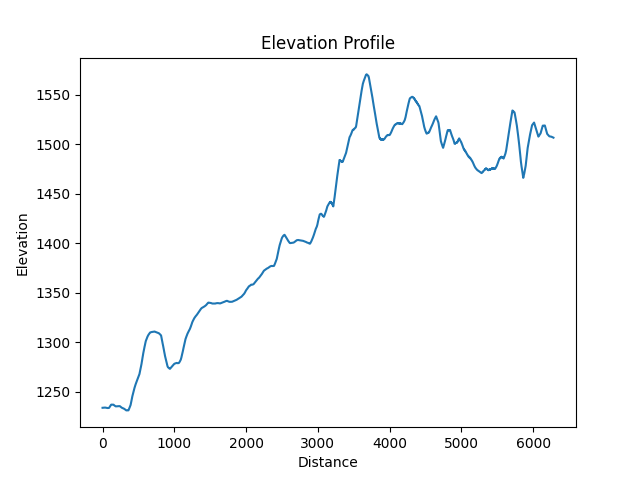
\includegraphics[width=0.3\linewidth]{elevation.png}
\caption{Plot over line \label{PlotOverCircularArcFigure}}
\end{figure}
\end{textblock*}
\end{frame}

\begin{frame}[fragile]
\begin{textblock*}{350pt}(50pt, 10pt)
\begin{block}{Acknowlegment}
I would like to thank \href{https://github.com/orgs/pyvista/teams/developers}{PyVista developer team} for developing useful library.
\end{block}
\begin{block}{References}
C. Bane Sullivan and Alexander Kaszynski, (2019). PyVista: 3D plotting and mesh analysis through a streamlined interface for the Visualization Toolkit (VTK). Journal of Open Source Software, 4(37), 1450, \url{https://doi.org/10.21105/joss.01450}
\end{block}
\begin{block}{Contact Information}
If you want to know and discuss pyvista more, join \href{http://github.com/pyvista/pyvista/discussions}{GitHub Discussion}.
\end{block}
\note{I would like to thank PyVista developer team for developing useful library.}
\note{If you want to know and discuss pyvista more, join \href{http://github.com/pyvista/pyvista/discussions}{GitHub Discussion}.}
\doclicenseThis
\end{textblock*}
\end{frame}

\end{document}

